% Chapter 5

\chapter{Galaxy Pairs, Mergers, and Morphologies} 
\label{Chapter:GalPairs}
\lhead{Chapter 5. \emph{Pairs, Mergers, and Morphologies}} 

\section{Background}

$\Lambda$CDM cosmology predicts the hierarchical assembly of dark matter haloes.
Throughout the history of the Universe haloes have grown in mass and size via two pathways. 
Firstly, haloes grow via smooth accretion gradually accreting dark matter from the surrounding environment. 
The secondary growth mechanism is via the accretion and gradual absorption of smaller haloes, known as subhaloes. 
After accretion subhaloes survive as substructure of the central/host halo, gradually losing mass and sinking to the centre of the potential well though dynamical friction. As discussed in previous Chapters, these subhaloes contain satellite galaxies that follow the halo structure resulting in galaxy-galaxy mergers.

Frequent or massive mergers are thought to induce morphological changes in galaxies. 
Galaxies, after experiencing a massive merger, where the minor galaxy is at least a quarter of the mass\footnote{Galaxy merger timescales far eclipse the human lifespan so the merger mass ratio is not an empirical constraint instead inferred from hydrodynamical merger simulations. It is somewhat free in simulations and can be used to tune to morphological fractions.} of the central galaxy, are thought to lose their disk-like morphology and transform into elliptical galaxies \citep{Negroponte1983SimulationsGalaxies, DeLucia2006TheGalaxies}. 
For this reason it is important to understand the frequency and nature of mergers between galaxies to achieve a complete and coherent picture of galaxy formation and evolution. 
Unfortunately, galaxy mergers occur on gigayear timescales and therefore it is not possible to directly observe the rate or consequence of galaxy mergers. 
The traditional approach to estimate the rate of galaxy mergers is to count galaxy pairs, and then assign a merging timescale to infer the rate \citep{Conselice20033,Conselice2008TheField,Mundy2017A3.5,Duncan2019ObservationalFields}.
A galaxy pair is usually defined by a mass ratio and a separation. For example, typical choices employed by observers are selecting galaxies that are within 5 to 30 kpc and fit the major merger criteria (1/3 mass ratio).
However, the approach of counting pairs is complicated by systematic differences when selecting galaxies. For example, the evolution of the pair fraction appears to change if a selection is made by flux ratio or made by stellar mass ratio \citep{Man2016RESOLVING03}.

\section{The systematic effects of stellar mass estimation on galaxy pair fractions}

%What systemeatics can we expect to find in galaxy pairs (paper 3 plots 1,2,&3)

In this chapter we show how different SMHM relations generate distinct pair fractions and by association different merger rates. 
Stellar mass functions with greater number densities of high-mass galaxies map larger galaxies into smaller haloes, resulting in steeper high-mass slopes for the SMHM relations.
In Figure \ref{fig:MassRatioCartoon} we show an illustrative cartoon of how different SMHM relations affect the galaxy mass ratios. 
For two identical halo pairs we see that a SMHM relation with a steeper slope causes a substantial difference in the stellar mass ratio that is mapped into the halo pairs when compared to a shallower SMHM relation. 

\begin{figure}[h]
	\centering
	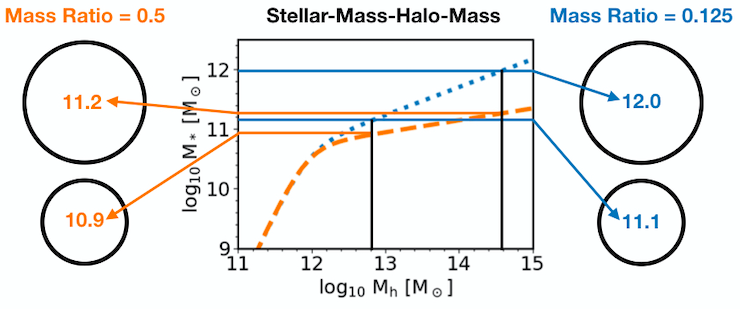
\includegraphics[width = \linewidth]{Figures/Chapter5/MassRatioCartoon.png}
	\caption{A cartoon showing how the SMHM relation impacts the stellar mass ratio of galaxies mapped into identical haloes. The steeper SMHM relation creates a smaller stellar mass ratio as the change in halo mass maps to a much larger stellar mass difference.}
	\label{fig:MassRatioCartoon}
\end{figure}

It follows that given two identical distributions of haloes seeded with galaxies via different SMHM relations the shallower one will seed more galaxy pairs\footnote{The pair fraction is defined here, in relation to major mergers, as the fraction of galaxies of a given mass that have a companion with a mass equal to or greater than a quarter of the primaries mass within 5-30 kpc.}.

In Figure \ref{fig:SMHM_PF_Cartoon} we show an example of systematic difference expected in the pair fraction when changing the SMHM relation.
The left-hand column shows the SMHM relations and the right column the pair fractions and their evolution with redshift. 
In the top row we compare two high mass slopes, one steep and one shallow, where the slope has been changed at redshift $z = 0.1$.
In the bottom row the slope at redshift $z = 0.1$ is fixed and we compare an evolving and non-evolving high-mass slope.

\begin{figure}[h]
	\centering
	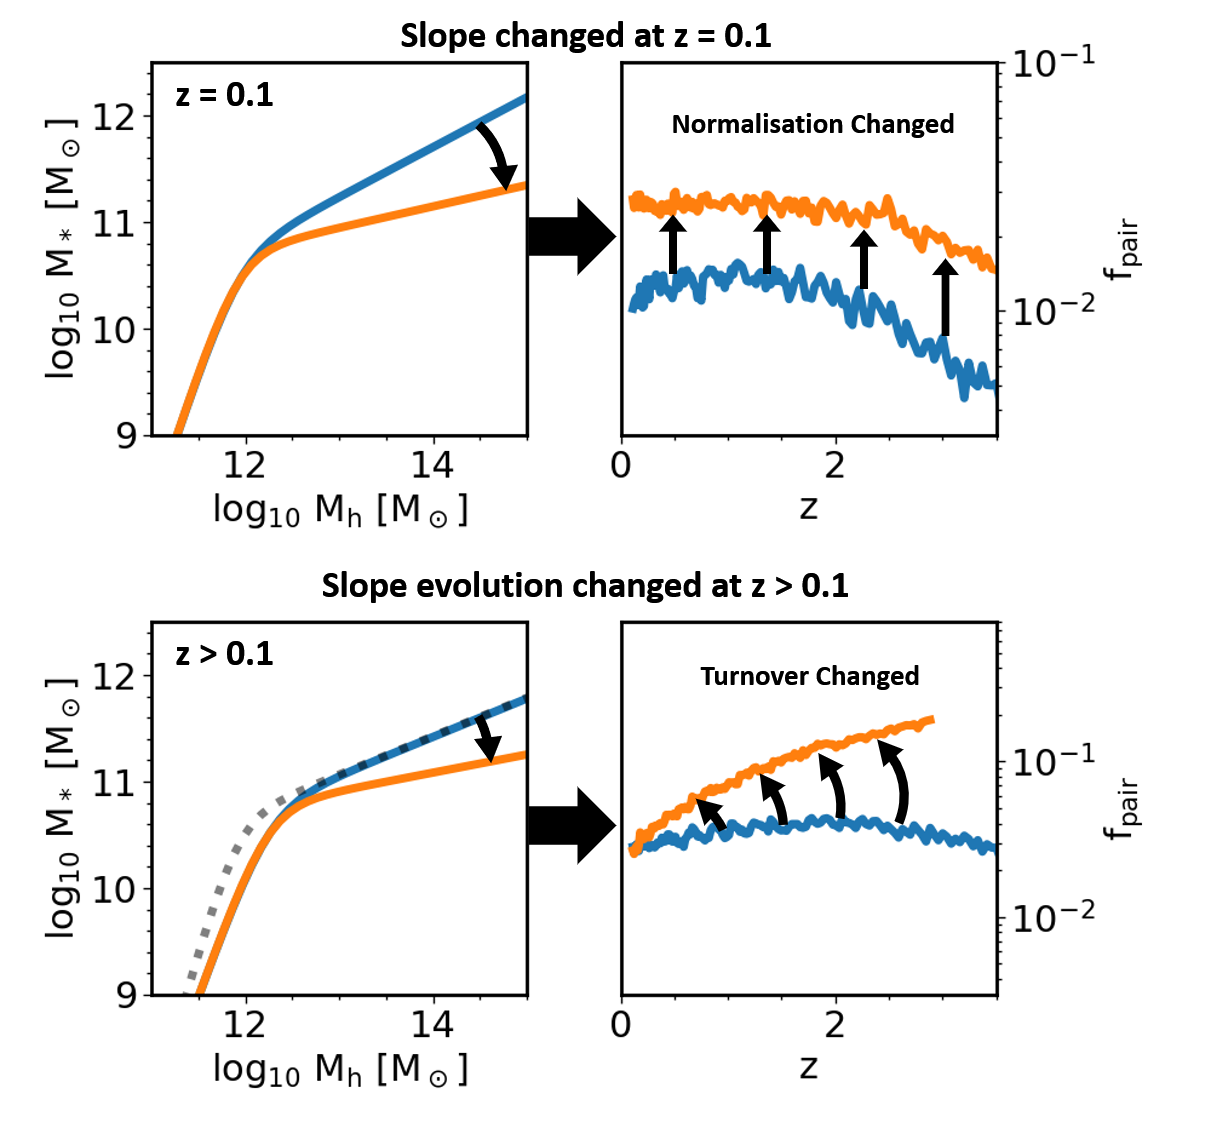
\includegraphics[width = \linewidth]{Figures/Chapter5/SMHM_PF_Cartoon.png}
	\caption{A cartoon showing how the SMHM relation can impact the pair fraction of galaxies with a mass ratio > 1/4. The top row shows how reducing the high mass slope of the SMHM relation increases the number of pairs at all redshifts. The bottom row shows the redshift $z=0.1$ relation as a grey dotted line alongside two evolving relations at redshift $z=2$ where one relation is evolved to be shallower (orange lines) compared a relation in remains steeper (blue lines). For the SMHM relation that evolves to be shallower, the pair fractions are found to increase. In each case the reason for the increase can be explained via Figure \ref{fig:MassRatioCartoon}, which shows that shallower SMHM relations produce a greater number of massive pairs. }
	\label{fig:SMHM_PF_Cartoon}
\end{figure}

The suppression of the high-mass slope increases the number of pairs created and the normalisation of the pair fraction increases. 
In the bottom row we show the effects of having a slope that flattens at higher redshift. 
We show the redshift $z=0.1$ relation in grey and the relations with the unchanged and changed slopes in blue and orange, respectively. 
The main effect of varying the evolution of the high-mass slope in the SMHM relation is to change the behaviour of the pair fraction with redshift. 
A steeper slope leads to a decreasing pair fraction, whereas a slope that gets shallower with time results in an increasing pair fraction.

The behaviours reported in Figure \ref{fig:SMHM_PF_Cartoon} are a direct consequence of the trends sketched in Figure \ref{fig:MassRatioCartoon}, where shallower slopes give higher fractions. 
Furthermore, from Figure \ref{fig:SMHM_PF_Cartoon} (and from Figure \ref{fig:PairFracSystematic}), it can be concluded that almost any pair fraction difference could be produced by appropriately altering the input SMHM relation. 
It is relevant to stress here that relatively minor changes in the stellar mass function can cause qualitative differences in the SMHM relation and, by extension, in the shape and normalisation of pair fractions at any cosmic epoch.

The ability to systematically change the pair fraction due to stellar mass derivation calls to question the discrepancies found in pair fraction results \citep[e.g.][]{Man2016RESOLVING03}. 
Systematic differences in the stellar mass measurements from different groups, will naturally yield different SMFs and thus, by extension, different SMHMs and pair fractions.  
\steel as a flexible and lightweight model can shed light on the extent of the systematics in the predicted pair fractions implied by different stellar mass estimates and SMFs, by running the same underlying cosmological model with the input SMHM relations corresponding to each distinct SMF.

Calculation of the pair fraction in \steel requires an estimate of the distance between the central galaxy and the satellite galaxy. analytic statistical DM accretion histories and not the outputs of a numerical simulation, we lack `physical' separations, we instead assign each subhalo bin an average distance to the central galaxy. 
The subhaloes start at the viral radius of the central halo, the distance to the centre then reduces directly proportionally to the amount of dynamical time elapsed \citep{Guo2011FromCosmology}, e.g. once half the dynamical time has elapsed the distance will be equal to half the starting distance.

In this chapter we investigate the impact on the distribution of satellites around central galaxies when using different SMHM relations. 
As this distribution is primarily dominated by the halo substructure, it is essential to make sure our selection criteria for galaxies always returns the same halo population. 
In a simulation with known haloes they can be directly selected select. However, to better match observation, where haloes are not known, the selection must be performed on an observable property.
As the stellar masses mapped into any given halo mass is a input and is therefore variable with halo mass it cannot be used. 
Instead, a constant number density selection can be made, selecting objects by abundance which theoretically will return the same halo population as we assume the halo structure to be a fixed quantity.
A similar technique was employed by, \citet[e.g.][]{vanDokkum2013The2.5, Huertas-Company2016MassCANDELS, Leja2013TRACINGSELECTION, Mundy2015Tracing3} to trace the evolution of galaxy populations. Galaxies at high redshift with a given comoving number density are assumed to be the progenitors of galaxy populations observed at later epochs with the same abundance. 
In this work we use a central stellar mass selection from the PyMorph stellar mass estimation of $M_{*} = 10^{11} - 10^{11.6} M_{\odot}$ (or $10^{9.5} - 10^{10.1} M_{\odot}$ when considering the low-mass slope controlled by $\beta$). For any given input SMHM relation we then select the galaxies that have a number density equal to the one corresponding to the aforementioned mass cut in the reference stellar mass function.
An example of this selection can be seen in Figure \ref{fig:PairFracSystematic}.
The shaded horizontal band shows the stellar masses for each SMHM relation with equal number density.

The SMHM relation is defined by 4(+4) parameters. We build a toy model where each of the parameters (M, N, $\beta$, $\gamma$), and their evolutionary factors (M$_z$, N$_z$, $\beta_z$, $\gamma_z$), are adjusted in turn to explore the effect on the galaxy pair fractions. Table \ref{tab:PairFracSysInput} details the change made to the SMHM relation for each parameter. 

\begin{table}
\centering
\caption{The adjustments to the SMHM relation used in Figure \ref{fig:PairFracSystematic}.}
\label{tab:PairFracSysInput}
\begin{tabular}{|c|cccc|} \hline
             & PyMorph   & $X_{0.1, alt}$  & $X_{z, +}$  & $X_{z, -}$  \\ \hline
$M$          & 11.92 & -0.25 & -     & -     \\ 
$M_{z}$      & 0.58   & -     & +0.1  & -0.1  \\ \hline
$N$          & 0.032 & +0.04 & -     & -     \\
$N_{z}$      & -0.014 & -     & +0.007 & -0.007 \\ \hline
$\beta$      & 1.64  & -0.3  & -     & -     \\
$\beta_{z}$  & -0.69  & -     & +0.3  & -0.3  \\ \hline
$\gamma$     & 0.53  & +0.06 & -     & -     \\
$\gamma_{z}$ & -0.03  & -     & +0.2  & -0.2  \\ \hline
\end{tabular}
\end{table}

Figure \ref{fig:PairFracSystematic} shows each of the SMHM relations in the outer four panels. The reference SMHM relation derived from the PyMorph photometry is depicted in blue at redshifts $z = 0.1$ (dotted line) and $z = 2$ (dashed line) in each panel. The modified redshift $z = 0.1$ relation is then shown in orange, and the increased and decreased (dashed red and green) evolution relations are plotted at redshift $z = 2$. The inner four panels show the results on the pair fraction and follow the same colour convention. 

\begin{landscape}
\begingroup
\begin{figure}[h]
	\centering
	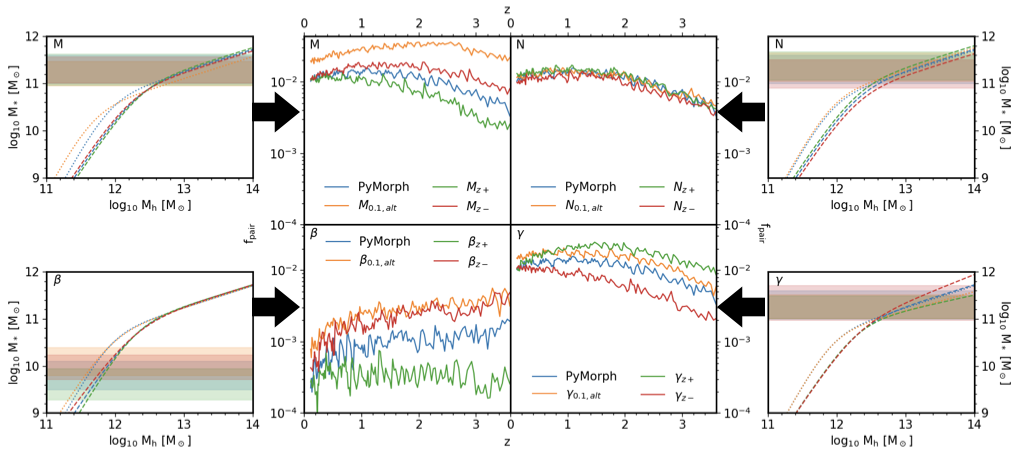
\includegraphics[width = \linewidth]{Figures/Chapter5/PairFractionSystematic.png}
	\caption{Each of the panel pairs (M, N, $\beta$, $\gamma$) shows the input SMHM relation in the outer plot and the modelled pair fraction evolution in the centre plot. Each pair investigates adjustments to the given parameter of the SMHM relation (M, N, $\beta$, $\gamma$). Each pair shows the reference SMHM relation `G18' in blue, the relation adjusted at redshift $z = 0.1$ keeping the same SMHM relation evolution parameters in yellow. The red and green lines have the evolution parameter altered such that the evolution parameter is increased or decreased with respect to PyMorph respectively. In the outer (SMHM relation) plots, dotted lines are $z = 0.1$ relations and dashed lines are $z = 2$ relations. The PyMorph relation is shown at both epochs for comparison. Finally, the shaded bands in the outer plots show the consistent number density selections used in the centre plots.}
	\label{fig:PairFracSystematic}
\end{figure}
\endgroup
\end{landscape}

When changing M, the knee parameter, a large increase in the pair fraction is found from a lower knee: The shallower high mass slope is extended, therefore more haloes are seeded in the mass range for pair selection. 
We see the same effect at high redshift, the lower value of M creates a higher pair fraction. 
The normalisation parameter, N, creates little change in the pair fraction as expected because the mass ratios are largely unaffected. 
The low mass slope parameter, $\beta$, affects the seeding of smaller galaxies hence a lower mass range is used for the consistent number density cut. 
Due to the steepness of the low-mass slope, the fraction of pairs found is lower in this mass cut.
Finally, when the high-mass slope parameter, $\gamma$, is altered, more pairs are found at high and low redshift when the slope is shallower. 
This is again attributed to more galaxies seeded within the mass ratio range.

\subsection{Comparison to simulation and observational results}
\label{subsec:SimObsRes}
The observed pair fraction is known to have discrepancies based on the galaxy property used to calculate the ratio. In \citet{Man2016RESOLVING03} it is shown that selecting pairs by flux ratio or stellar mass creates differences in the pair fraction evolution. 
In Figures \ref{fig:MassRatioCartoon} \& \ref{fig:SMHM_PF_Cartoon} we show the predicted effect of the determination of stellar mass on the SMHM relation and the systematic propagation of these changes into the pair fraction. 
Through the use of a toy model, in Figure \ref{fig:PairFracSystematic} we show how isolated perturbations to the eight SMHM relation parameters propagate into the galaxy pair fraction.
From this analysis we conclude that any measurement of the pair fraction is strictly related to the underlying assumptions on stellar mass measurements. 
Our findings thus imply that meaningful comparisons between different pair fraction measurements can only be undertaken under identical stellar mass derivation assumptions, or where this is not the case the influence of any differences are accounted for.
In this section we fit, by making use of $\steel$, observed pair fractions using small changes to the SMHM relation.
We anticipate this modelling can be used to provide corrections to pair fraction results to allow for more meaningful comparisons.

\subsubsection{Simulation: Illiustris TNG}

In Figure \ref{fig:PairFractionIll} we show the simulated galaxy pair fractions for galaxies in the mass range $M_*$ = $10^{10}M_{\odot}$ to $10^{10.6}M_{\odot}$. The pair fraction is shown for two different SMHM relations used as inputs to $\steel$. In blue we show the PyMorph (S\`ersic-Exponential) input used as the reference in Figure \ref{fig:PairFracSystematic}, in orange the input SMHM relation is calibrated to match outputs of the Illustris TNG simulation. In the right-hand panel we see that pair fraction predicted by STEEL using in input the SMHM relation calibrated on TNG, is in good agreement with the pair fraction extracted directly from the Illustris TNG simulation. This is a valid test that lends further support on the ability of STEEL to generate robust pair fractions for a given input SMHM relation. The pair fraction predicted using the PyMorph input is 0.5 dex lower. This is expected as in the mass range we are considering the Illustris TNG simulation SMHM relation is shallower and more pairs are therefore created in a greater mass range of halo mergers. 
\begin{figure*}
	\centering
	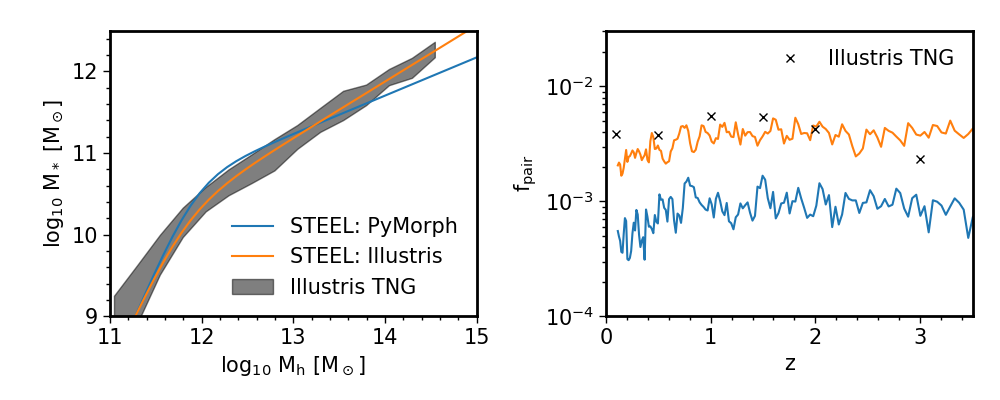
\includegraphics[width = \linewidth]{Figures/Chapter5/PairFractionIllustris.png}
    \caption{Left: Two SMHM relations are shown from \steel using parameters designed to reproduce the SMHM relation found in the Illustris TNG simulation (Orange line) and the PyMorph (S\`ersic-Exponential) fit parameters (Blue line). The shaded region is the output from the Illustris TNG simulation. Right: The pair fractions predicted by STEEL for galaxies in the mass range  $M_*$ = $10^{10}M_{\odot}$ to $10^{10.6}M_{\odot}$  from the two input SMHM relations plotted in the left panel (same colour coding). The black crosses indicate pair fractions directly extracted from the Illustris TNG simulation.}
	\label{fig:PairFractionIll}
\end{figure*}

\subsubsection{Observation: \citet{Mundy2017A3.5}}

To further investigate the variations of pair fraction when varying the input stellar mass estimates and therefore the SMF, we compare the predicted pair fraction evolution using two SMHM relations. Specifically we use the SMF presented in Section \ref{C2:SubSec:AbnMtch}, PyMorph and cmodel. PyMorph has a substantially greater number of high mass galaxies and thereby produces a steeper SMHM relation.
In Figure \ref{fig:PairFractionData} the left-hand panel shows each SMHM relation at redshift $z = 0.1$ and $z = 2.5$. Following the systematic investigation in Figure \ref{fig:PairFracSystematic}, we attribute the 0.1 dex difference in pair fraction to the difference in high mass slope between PyMorph and cmodel. The best-fit relation from \citet{Mundy2017A3.5}, shown as black crosses, rises at eairler cosmic epochs rather than falling; as seen from PyMorph and cmodel. We saw in Figure \ref{fig:PairFracSystematic} that a SMHM relation with a high-mass slope decreasing with redshift will generate a pair fraction evolving similarly with redshift.

\begin{figure*}
	\centering
	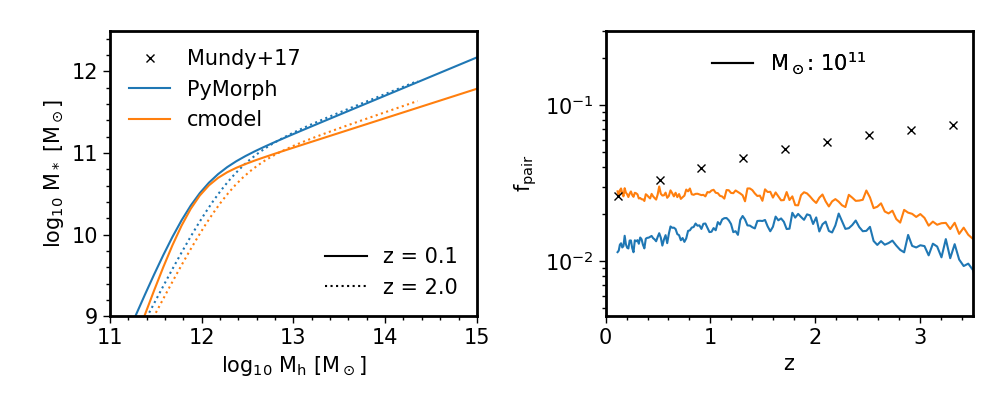
\includegraphics[width = \linewidth]{Figures/Chapter5/PairFractionData.png}
    \caption{Left: Stellar-mass-halo-mass relations derived from PyMorph (blue) and cmodel (orange) at redshifts $z=0.1$ (solid lines) and $z=2.0$ (dotted lines). Right: The pair fraction evolution for galaxies using both SMHM relations. The black crosses show the corresponding best fit for the $>10^{11}M_{\odot}$ mass cut from \citet{Mundy2017A3.5}.}
	\label{fig:PairFractionData}
\end{figure*}

In an attempt to reproduce the \citet{Mundy2017A3.5} pair fraction evolution with redshift we begin using the cmodel SMHM relation which gives the closest match to \citet{Mundy2017A3.5} in pair fraction at low redshift. Following the analysis of Figure \ref{fig:PairFracSystematic}, where higher $\gamma_{z}$ increases the pair fraction at high redshift, we alter the parameter from 0.0 to 0.5 in steps of 0.1. In Figure \ref{fig:PairFractionHMevo} the left panel shows the SMHM relation at redshift $z=0.1$ as a black dotted line, while the coloured lines show the relation at redshift $z = 2$ with different $\gamma_{z}$ parameters. The right panel shows the impact of this evolution on the pair fraction. As predicted higher $\gamma_{z}$ increases the pair fraction with redshift and a value of above 0.1 removes the turnover. Comparing to \citet{Mundy2017A3.5} we see a value of $\gamma_{z}$ between 0.1 and 0.2 best reproduces the rise in pair fraction. 

\begin{figure*}
	\centering
	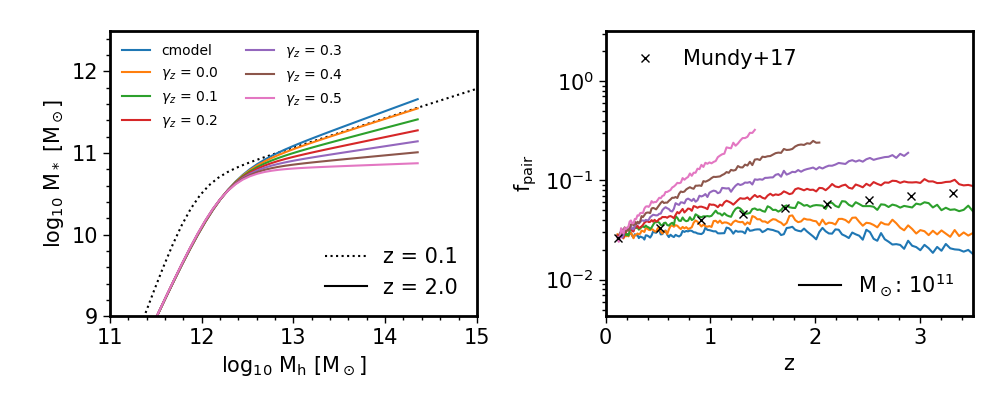
\includegraphics[width = \linewidth]{Figures/Chapter5/PairFractionHMevo.png}
    \caption{Left: Stellar-mass-halo-mass relations derived from cmodel (black) at redshift $z = 0.1$ (dotted lines) and at $z = 2.0$ with altered high mass-slope evolution parameter (coloured lines). Right: pair fractions corresponding to the SMHM relations plotted in the left panel (same colour coding). The black crosses show the best fits for the $>10^{11}M_{\odot}$ mass cut from \citet{Mundy2017A3.5}.}
	\label{fig:PairFractionHMevo}
\end{figure*}

\section{Galaxy Morphologies Resulting from Galaxy Mergers}
%What happens during a galaxy merger?

Mergers are thought to be one of the drivers for morphological transformation, size growth and other structural and dynamical changes in galaxies \citep{Bournaud2007, Hopkins2009TheDemographics, Hopkins2010MergersFunctions, Shankar2011SizeUniverse, Fontanot2015OnMergers}. A number of analytically-based cosmological models have generally assumed that major mergers in particular, with a mass ratio of at least $M_{sat}/M_{cen} > 0.25$ (to 0.3), are effective in destroying disks and in forming ellipticals \citep{Baugh2006AApproach, Malbon2007BlackFormation, Bower2010TheFormation}. However, galaxy mergers occur on megayear or even gigayear timescales therefore observations of galaxy mergers are essentially static snapshots of the processes. Most of our knowledge of galaxy mergers comes from analysis of simulations of merging systems \cite[e..g.][]{Hopkins2006ASpheroids,Hopkins2009TheDemographics, Hopkins2010MergersRate,Hopkins2009HOWMERGERS,Hopkins2010MERGERSMATTER,OLeary2020EMERGE:zsim6,Fensch2017High-redshiftFormation,Stewart2008MergerSurvival,Stewart2009GALAXYDEPENDENCE}. 

Despite the wealth of simulations of galaxy mergers, the fulcrum of our understanding of how mergers affect the galaxy population lies with the estimation of the merger rate and significance of mergers \cite{Hopkins2010MERGERSMATTER, Hopkins2010MergersRate}. Using the merger rates derived in Chapter \ref{Chapter:GalGrowth} we implement a post-processing method to ascertain the effects of traditional mergers models when applied to true, statistical, populations in $\steel$.

%The fraction of elliptical galaxies stemming from galaxy major merger in steel
\subsection{Implementing discrete processes in a statistical model.}

One of the primary challenges in the development of \steel is trying to implement discrete processes in a statistical fashion. Mergers between two galaxies are implemented stochastically using the following method.
\begin{itemize}
    \item At each time-step, for each central halo mass track, the mass bins of previously accreted subhalo/satellite galaxy mass functions that have reached the end of their dynamical time, are summed to produce the merging satellite stellar mass function. 
    \item Each central halo mass track is assigned a central stellar mass at each epoch $M_{*,cent}(M_{h}, z)$ (Figure \ref{fig:Cent_Mass_PP}). By integrating the merging satellite stellar mass function in the range [$M_{*,cent}(M_{h}, z) \cdot \mu$, $M_{*,cent}(M_{h}, z)$] the probability that a given central has undergone a major merger at each epoch is retrieved, where $\mu$ is the major merger mass ratio. 
    \item In Figure \ref{fig:Gal_Morph_toon} an illustration of the way galaxy morphologies are updated is given. 
    \begin{itemize}
        \item In the leftmost panel all galaxies are spirals or a disk like morphology (blue bar). The probability of a galaxy having a major merger is shown as a black line.
        \item Following the arrow to the middle panel the fraction of galaxies that had a major merger are assigned as ellipticals. The mass track at this epoch now has this spiral to elliptical ratio.
        \item At the next time step the fraction of galaxies undergoing a major merger is calculated. However, this fraction is split between galaxies that have previously had a major merger and those that have not. 
        \item Only the galaxies that were in the spiral group in this time step contribute to the increasing elliptical fraction.
        \item Repeating this procedure at each time-step eventually all galaxies may have the potential become elliptical but the rate at which this happens progressively slows in time due to the decreasing spiral population.
    \end{itemize}
\end{itemize}

\begin{figure}[h]
	\centering
	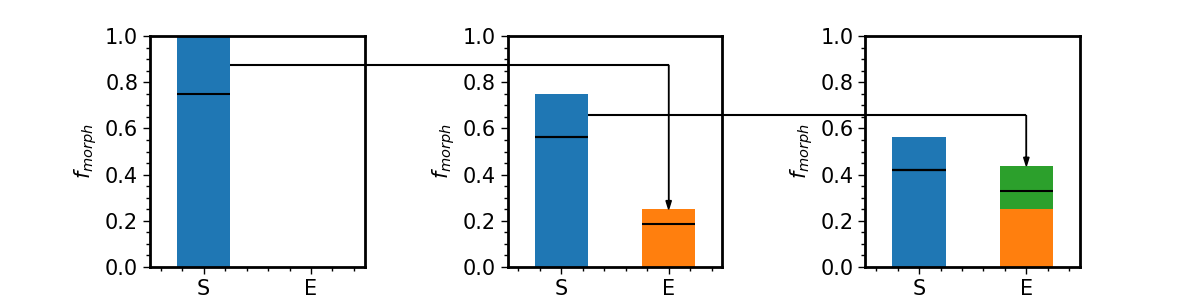
\includegraphics[width = \linewidth]{Figures/Chapter5/Morphology_Evolution.png}
	\caption{A cartoon to show the way we assign morphologies statistically in $\steel$. Each step has the same fraction of major mergers but the number of ellipticals created reduces as some major mergers occur on the elliptical fraction. The fraction of galaxies in each population experiencing a major merger is displayed as a horizontal black line.}
	\label{fig:Gal_Morph_toon}
\end{figure}

Applying the above process to galaxies in \steel from redshift $z = 3$, we build the morphological fraction of galaxies at different masses using a major mass ratio of $\mu = 0.25$, at redshifts $z = 0.1, 0.65, 1.75$. Figure \ref{fig:Gal_Morph} shows the probability/fraction of central galaxies that have elliptical morphologies, while the black triangles show the T-Type-selected elliptical fraction from the SDSS catalogue at redshift $z = 0.1$. We find that applying this simple recipe to the merging number densities from \textsc{steel} creates a good match to the elliptical fraction in the local universe.

\begin{figure}[h]
	\centering
	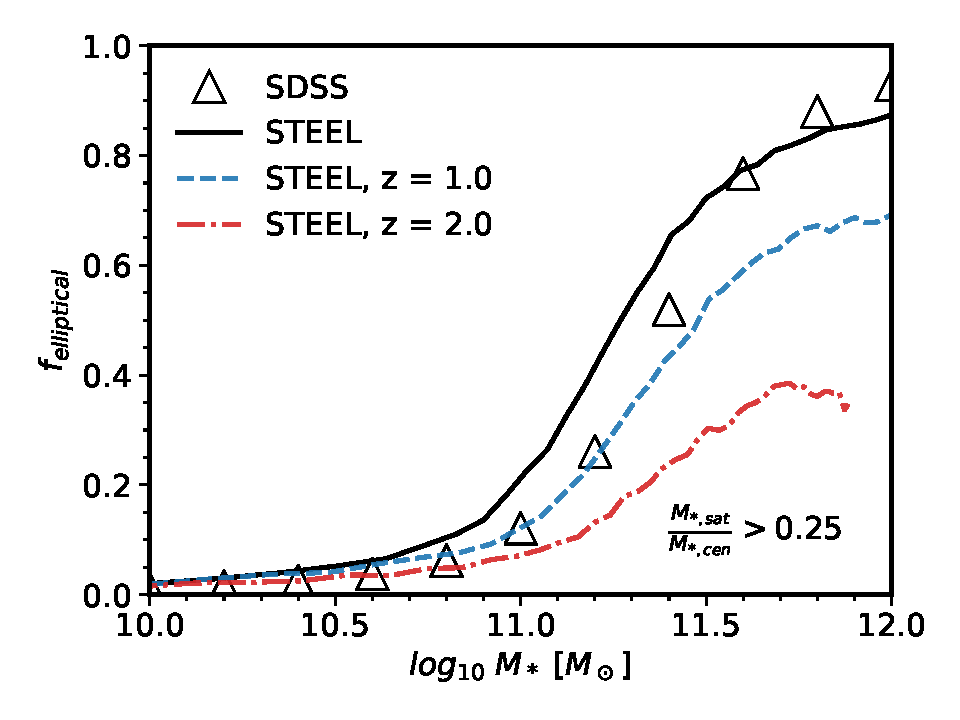
\includegraphics[width = \linewidth]{Figures/Chapter5/GalaxyMorphologies.pdf}
	\caption{Fraction of ellipticals as a function of stellar mass predicted by STEEL at three different redshifts, as labelled. The triangles are the T-Type selected elliptical fraction from SDSS at redshift $z = 0.1$.}
	\label{fig:Gal_Morph}
\end{figure}


\section{Lenticular Galaxy Formation}
%What is a lenticular and why are they considered independently to the rest of the galaxy population?
Lenticular galaxies are categorised by their unusual appearance. In the famous `tuning fork' diagram derived by \citet{Hubble1927TheNebulae}, the lenticular galaxies are found where the two spiral `forks' meet the elliptical `handle'. Lenticulars similarly to spirals have an extended disk but do not boast the `bars' or `arms' that decorate the disks of spiral galaxies nor the resiviors of cold gas suitable for star formation \cite{CHAMARAUX1986TheSamples}; similar to ellipticals lenticulars have a velocity dispersion-dominated bulge at their centre. 
%What have been the proposed models of Lenticular formation?

Given that are morphologically and dynamically positioned in between spirals and massive ellipticals, it is reasonable to assume that they may have arisen on the transformation pathway between the two populations. The latter hypothesis is further corroborated by the observational evidence that lenticulars \cite{Dressler1980GalaxyGalaxies}, and the fraction of lenticulars increases with decreasing redshift simmilarly to that of ellipticals \cite{Postman2005TheClusters}. 

%Building a least assumption model of lenticular formation (supervised project)
\subsection{Lenticular formation in empirically constrained environments.}
\textit{The work presented in this subsection was carried out by SP under the supervision of PJG and FS. The direction of the project was heavily influenced by PJG and builds upon the successes found in predicting morphologies in \steel.}

Given the successes in ratifying the simple merger model of elliptical formation within $\steel$, we extend the predictions of STEEL to lenticular galaxies. We emply an additional assumption (and related parameter) in the model inspired by relevant proposal in the literature, and compare with SDSS data.

\subsubsection{\citet{Cook2009Two-phaseFormation} Model}

We started our investigation by implementing the lenticular formation model by \citet{Cook2009Two-phaseFormation}. This model divides halo growth into two distinct phases: \begin{itemize}
    \item A fast collapse and intense merging phase at high redshift.
    \item A slow accretion phase at low redshift after a transition epoch $z_{t}$.
\end{itemize}
Following this two-phase halo growth,the central galaxy first form a bulge during the fast collapse phase, and then gradually form a stellar disk around it in the second phase. The model for building spheorids in this semi-analytic model is the same as that implemented in \citet{Granato2004AHosts}. 

Translating semi-analytical techniques into a statistical-semi-empirical model by nature of the two models results in a loss of complexity. In order to maintain the core prediction of the \citet{Cook2009Two-phaseFormation} model we focus on the two phase formation aspect as follows. Galaxies are selected where they have grown a significant fraction of their mass (e.g. 70\%) between two epochs as assigned as lenticulars. These galaxies can then undergo further evolution by being transformed into ellipticals as described by the merger model from the previous section. Despite exploring a large parameter space in the mass fraction and redshift thresholds, we still find that within the framework given by \steel, the \citet{Cook2009Two-phaseFormation} model can not reproduce the SDSS measured lenticular fractions, as illustrated in Figure \ref{fig:CookeModel}.

\begin{figure}
  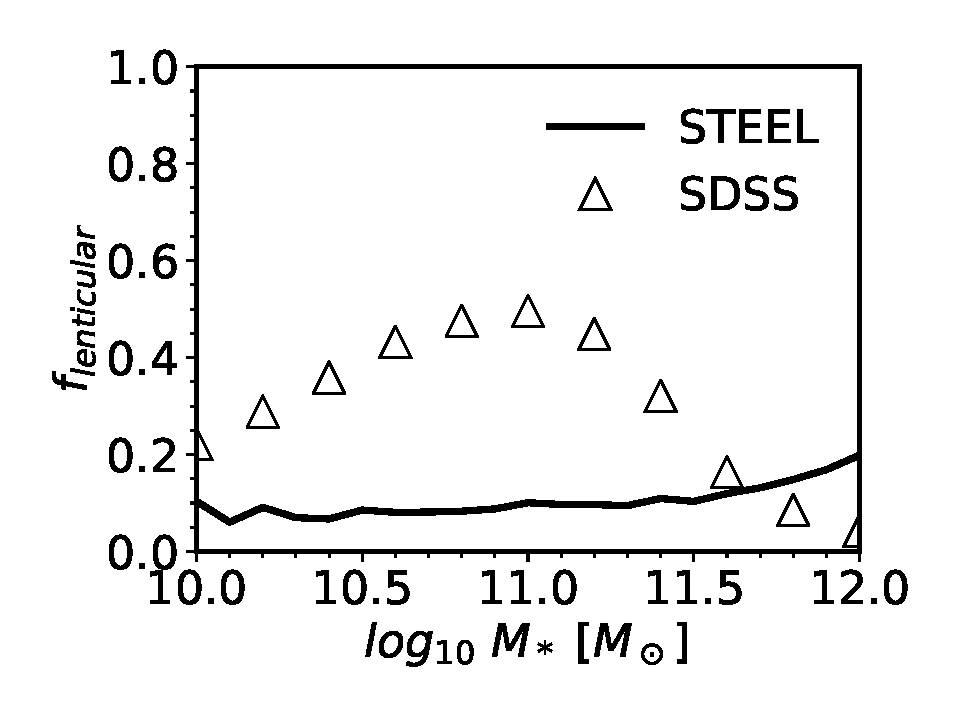
\includegraphics[width=\linewidth]{Figures/Chapter5/CookModel.pdf}
    \caption{The solid line mark the lenticular galaxy fractions generated using a simplified version of the lenticular formation method described in
    \cite{Cook2009Two-phaseFormation}. The model assumes lenticular galaxies are those that have formed a significant fraction of their stellar mass during a particular epoch. However, even after significant optimisation of the mass
    threshold and epoch definitions, it is never possible to reproduce the SDSS
    data (open triangles) within \steel using this model.}
    \label{fig:CookeModel}
\end{figure}

\subsubsection{Minimal assumption model}

Given the unsuccessful implementation of the \citet{Cook2009Two-phaseFormation} model, we revisit other proposed models to find out which (or a set of) have the potential to generate the observed lenticular fraction. Considering the nature of lenticulars in observations, which increase their fraction with decreasing redshift in a similar fashion to ellipticals \cite{Huertas-Company2015TheGrowth,Huertas-Company2016MassCANDELS} the first model we implement extends that of the elliptical merger model. An additional merger mass threshold ($\mu$) is implemented at $\mu = M_{*, sat}/M_{*, cen} = 0.05$. Central galaxies that experience a merger between this mass threshold and the major merger threshold are assigned to be lenticulars, while the central galaxies with mu>0.25 are still converted into ellipticals. Lenticular galaxies that subsequently experience mergers above the major mass ratio are then reassigned as ellpticals. This essentially adds a central 3rd column to Figure \ref{fig:Gal_Morph_toon}. As can be seen in the first panel of Figure \ref{fig:Lentcular_panels} this simplistic model over-produces lenticulars in the high mass end. 

To reduce the lenticular production at high masses, following similar ideas to the gas dissipation models utilised in \citet{Hopkins2009}, we test a hard gas threshold. Physically this gas threshold can be interpreted as a damping force, the gas dissipates the energy of the merger into heating the gas reservoir limiting the disruption to the galaxy structures. Initially, only galaxies with a gas fraction above the threshold can be converted into lenticulars. As shown in the middle panel this removes all lenticulars from the high mass end where galaxies tend to be gas poor. 
Finally, to improve the fit to the data we implement a `soft' gas fraction, according to which galaxies below a given mass fraction become statistically less likely to become lenticulars after experiencing a major merger. We include the soft gas threshold to reflect the varying efficiency of gas at different fractions dissipating the energy. This combination of models well fits the high-mass lenticulars as can be seen in the rightmost panel of Figure \ref{fig:Lentcular_panels}.

\begin{figure}
  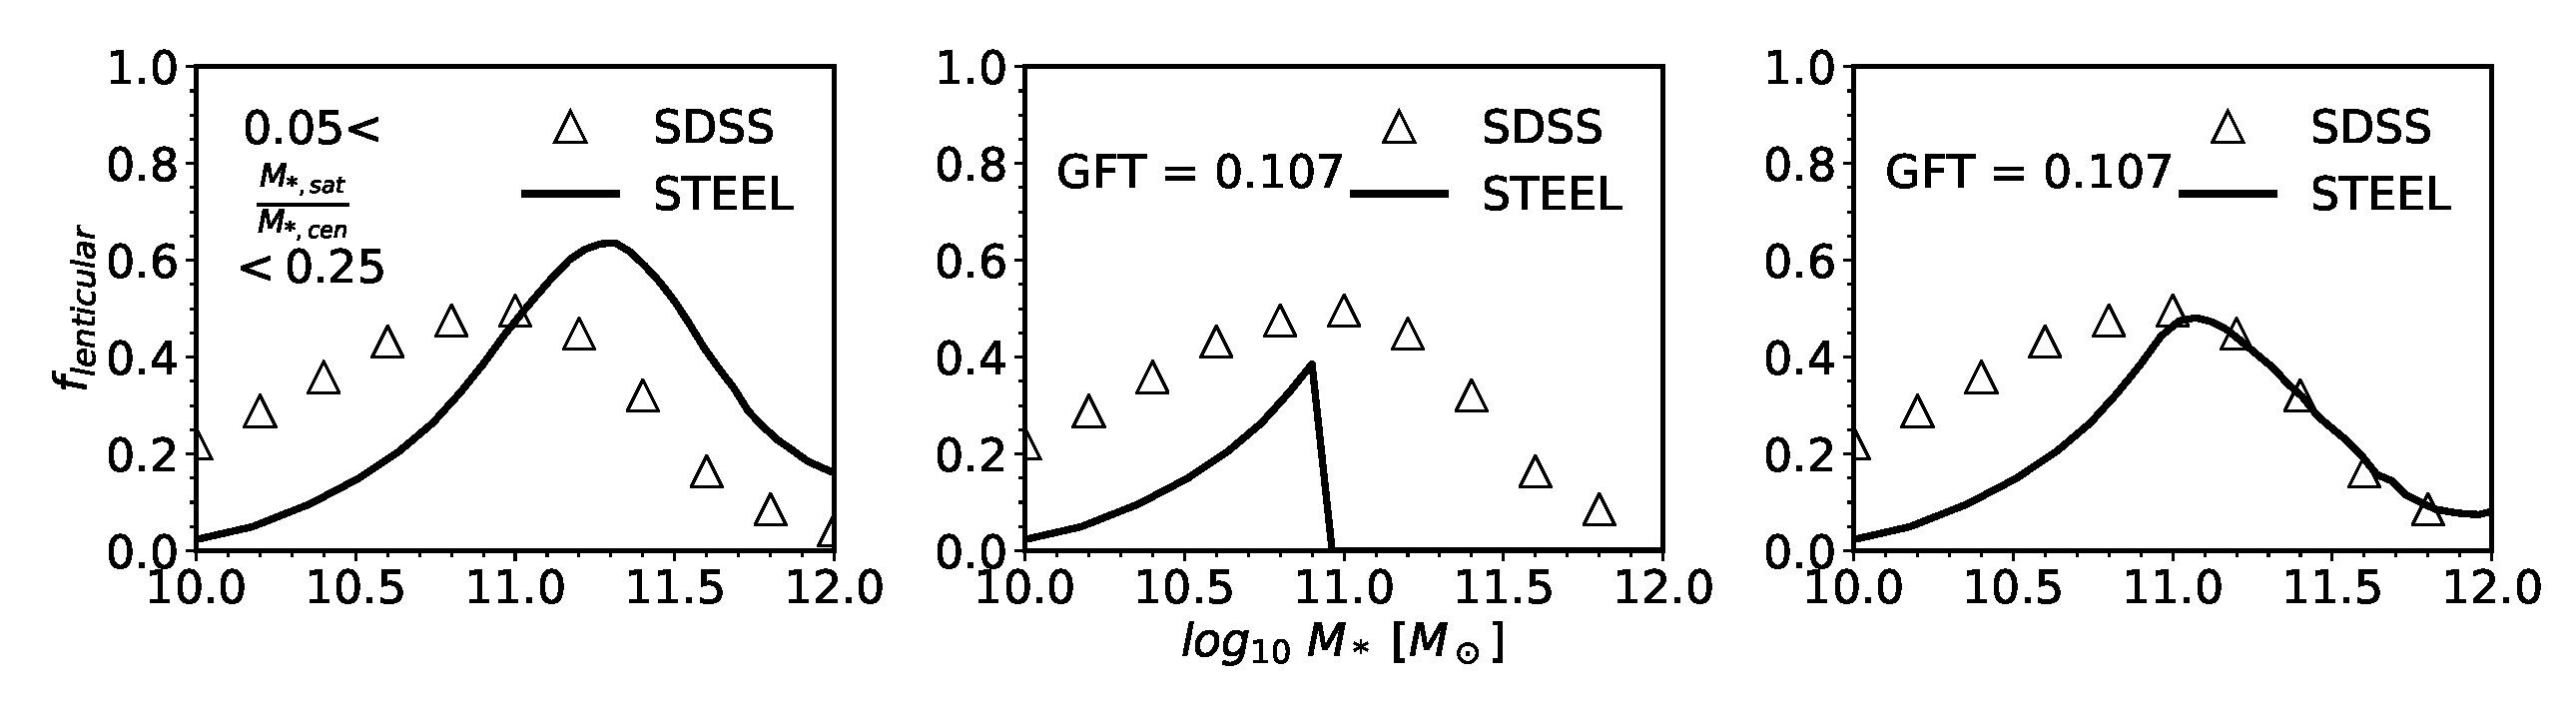
\includegraphics[width=\linewidth]{Figures/Chapter5/Lenticular_three.pdf}
    \caption{Three plots from left to right show lenticular fractions generated using the merger model with different parameters and variants. The first (leftmost) panel shows the fraction generated by summing the number densities of merging galaxies with mass ratio in the range $0.05 < \mu < 0.25$. The middle panel shows the effect of adding a hard gas ratio cutoff to the merger model, galaxies that are below a gas fraction threshold (GFT) do not form lenticulars. Finally, changing the model to a `soft' gas fraction threshold where the efficiency of lenticular formation is reduced above the GFT.}
    \label{fig:Lentcular_panels}
\end{figure}

Lower mass galaxies reside in less rich environments and grow more via secular (in-situ) processes. It is therefore expected that the merger/dissipation model will not significantly contribute to the formation of lenticulars at these masses. To build lenticulars at these masses we implement a disk instability model following the baryonic inflow rates given by \citet{Bournaud2011BLACKSTREAMS}. During their continuous growth in stellar mass along cosmic time, we allow galaxies to build their central bulges through gas transport from the disk using Equation \ref{eqn:DiskInflow} the analytic approximation of \citet{Bournaud2011BLACKSTREAMS} extracted from high-resolution hydrodynamic simulations, 

\begin{equation}
    \label{eqn:DiskInflow}
    \dot{M}_{inflow} = 25 log_{10}\Big[\frac{M_{*,disk}}{10^{11}M_{\odot}}\Big]\Big(\frac{1 + z}{3}\Big)^{1.5}.
\end{equation}

The mass of the bulge is then given by

\begin{equation}
    M_{bulge} = \sum_z \dot{M}_{inflow} \times \delta t(z).
\end{equation}

In each mass bin a fraction of galaxies proportional to the mass ratio of the bulge to the total stellar mass, $A \times M_{bulge} / M_{*, total}$, are added to the lenticular population. The resulting fit to the population is shown in Figure \ref{fig:All_Morphologies}.

\begin{figure}
  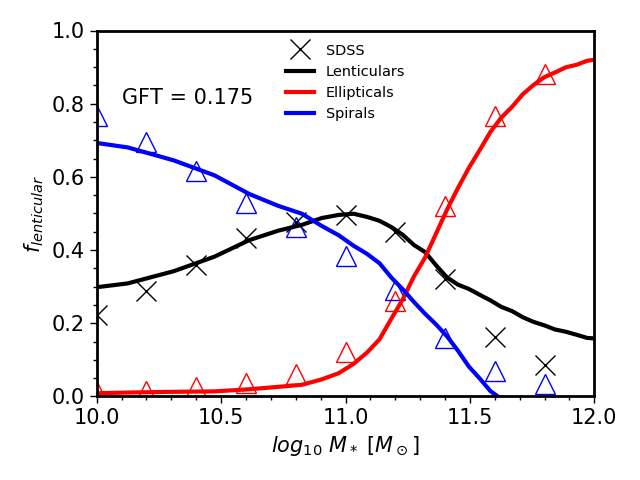
\includegraphics[width=\linewidth]{Figures/Chapter5/Bulge_Growth_Final_All_Morph.png}
    \caption{Fractions of different galactic morphological classes as a function of stellar mass. Ellipticals are generated using a major merger model, lenticulars using the combined merger (with soft gas fraction) and baryonic inflow models and, spirals are the remaining population. Models are compared to data from SDSS (symbols, as labelled).}
    \label{fig:All_Morphologies}
\end{figure}

We find the combination of a merger and inflow model is able to adequately recreate the lenticular fractions. This two channel model is potentially consistent with the distinct morphological types, barred and un-barred, found within the lenticular population \cite{Laurikainen2005MulticomponentGalaxies, VanDenBergh2012LuminositiesGalaxies}.

In summary, to recreate the lenticular population we find it necessary to add three assumptions/parameters in addition to the major merger mass ratio used to create the ellipticals. The first is the `minor' mass ratio limit that defines the minimium mass ratio at which lenticulars are formed via mergers, the second is the `soft' gas mass threshold that damps the creation of lenticulars, and finally, we need to allow for an additional channel of bulge growth via secular evolution, which, at variance with the merger channel, is particularly effective at lower stellar masses. 

\section{Discussion}

In this chapter we have shown two applications of $\steel$. Firstly, we prooved the ability of \steel to unravel the effects of systematics in stellar mass estimates in varying the implied galactic pair fractions. Secondly, we show an example of how constrained merger histories can be used to test the efficency of morphological evolution models reproduce the observed morphological fractions.  

\subsection{Pair Fractions}

The primary goal of the pair fraction analysis is to show the propagation of systematics in galaxy modelling. 
Specifically, we used the SMHM relationship to connect assumptions used when estimating observed stellar masses to systematics in galaxy pair fractions in the context of a \LCDM Universe. 
In this chapter we adopted as a reference two observed stellar mass functions from SDSS-DR7 observations that use a de Vaucoulers and a S\`ersic + Exponential fit to determine stellar masses, which in turn create stellar mass functions with notably different number densities at the high mass end. Each stellar mass function then generates, through abundance matching, a different SMHM relationship. The S\`ersic + Exponential mass function generates a steeper high-mass slope in the SMHM relationship at any epoch.
In addition to the SMHM relationships from the observed data we used a relationship fitted to match the outputs of the Illistris simulation. Furthermore, we also considered a toy model SMHM relation individually perturbing each input parameter to transparently probe the impact of the input SMHM relation on the pair fractions.
In each case we find that small changes introduced into the SMHM relationship can have significant effects on the expected pair fractions, as shown in Figures \ref{fig:MassRatioCartoon},\ref{fig:SMHM_PF_Cartoon}, \& \ref{fig:PairFracSystematic}.
This suggests that in the contxet of a \LCDM Universe tensions in previous observational studies could, in large part, be traced back to systematics in stellar mass estimates.

In \citet{Mundy2017A3.5} the $M_{*,cen} > 10^{10} M_{\odot}$ pair fraction is not significantly different from the $M_{*,cen} > 10^{11} M_{\odot}$ pair fraction shown in Figure \ref{fig:PairFractionData}. In Figure \ref{fig:PairFracSystematic} we find the pair fraction drops significantly when a mass selection is taken below the SMHM relation knee. As this drop is not found by \citet{Mundy2017A3.5} we interpret that their pair fraction measurement is not consistent with a break in the SMHM relation between $10^{10} M_{*,cen}$ and $10^{11} M_{*,cen}$.

\citet{Man2016RESOLVING03} noticed that the choice between luminosity-selected and stellar-mass selected pairs affected the pair fraction evolution. In this work we provided a clear framework to properly interpret how input choices create systematic effects in the observed pair fraction and its evolution. Furthermore, it is a common approach to infer the assembly history of galaxies by converting the pair fractions into merger rates by assigning timescales to galaxy pairs \citep{Conselice20033,Conselice2008TheField,Mundy2017A3.5}. 

In this Chapter we connected the shape and evolution of the SMHM relationship to the evolution of the pair fractions.
We proposed it is therefore possible to use the pair fraction as an additional constraint to the SMHM relationship. This is a natural extension of conditional abundance matching or extended SHAM (subhalo abundance matching) models \citep{Hearin2013SHAMGroups}.
Using $\steel$, one can test simultaneously the accretion ratio and the pair fraction generated from a given stellar mass function and cosmology.

Any changes to the stellar mass estimates such as photometry, background subtraction, IMF, e.t.c. that affect the stellar mass function in a given cosmology will create a change in the SMHM relationship. Therefore, by the systematic propagation demonstrated in this work, any stellar mass estimation will create systematic differences in the pair fractions. 
With the techniques presented throughout this thesis, one could retrieve the systematic differences created in pair fraction under multiple \LCDM cosmologies and for any given set of stellar mass functions. As a further test of the effectiveness of our methodology, we show showed that when inputting into STEEL the SMHM relation from the Illustris simulations, we are able to retrieve the pair fractions independently inferred from the same simulations.

In the era of wide and deep surveys, such as EUCLID, constraining a model using a single multi-epoch data set with consistent photometry will become a reality. The advantages of this are twofold: By tuning the SMHM relation to a given survey over a large range of redshifts, the growth of the stellar mass function over time can be tested against the implied satellite accretion and star formation rate as in Chapter \ref{Chapter:GalGrowth}. This can be seen as a consistency test of the cosmological model or of the consistency of the stellar mass and/or starformation rate estimations. Secondly, as in Chapter \ref{Chapter:GalDist}, one can test if the high redshift SMHM relation is consistent with the low redshift satellite distributions. Although, the constraints on a given photometry, cosmological model, satellite evolution, starformation rate, e.t.c... are still not complete, \steel will allow for non-physical results to be identified. Furthermore, by making the model accessible it can then be used in the manner described above to make systematic adjustments to compare between current and future data sets that may use different stellar mass estimations.

\subsection{Morphologies}

Given the very promising results of \steel in predicting satellite number densities in different environments and epochs, we here took a step further and explored whether \steel's cumulative number of major mergers is able to account for the local fraction of elliptical galaxies as well as implementing several lenticular formation models. 

Despite the noticeably good agreement between model predictions and data in Figure \ref{fig:All_Morphologies}, we stress that different input SMHM relations can, as shown in this Chapter \ref{Chapter:GalGrowth}, substantially affect the accretion rate which in turn will modify the number of galaxies experiencing major mergers. It follows that any cosmological galaxy evolution model that uses mergers as a physical driver for galaxy transformation should first simultaneously and self-consistently closely reproduce stellar mass functions, the SMHM relation, satellite distributions, and pair fractions at previous redshifts.

\section{Conclusions}
\label{sec:Conclusions}

In the first part of this Chapter, we showed that the input SMHM relations, based on different stellar mass estimations, have a significant impact on the predicted galaxy pair fractions. In short, the steeper the relation, the lower the predicted pair fraction. Specifically, we compare stellar mass functions created and a de Vaucoulers-based photometry (cmodel) to a S\'ersic-Exponential photometry (PyMorph), the latter leading to an enhancement in the number density of high mass galaxies. The resulting effect of these stellar mass functions is a different input SMHM relation to $\steel$, the primary difference consisting of a steeper high-mass slope when adopting the S\'ersic-Exponential profile. As expected, the S\'ersic-Exponential results in a lower pair-fraction. To attempt to explain the difference in pair-fraction evolution with redshift, we create a suite of toy models testing different alterations to the SMHM relation. We find that this evolution is linked to the evolution of the high-mass slope.

The purpose of this work is to show how subtle changes in the derivation of stellar mass could lead to large differences in the observationally-calibrated pair fractions. It is therefore crucial when comparing two different samples, to account for the systematic biases introduced by the different assumptions implicit in stellar mass estimation. Observations or models that do not accurately match the stellar mass function measured in the observational samples the compare to, will not be able to self-consistently reproduce results.

The second part of this Chapter focuses on the implementation and validation of popular morphological models into $\steel$. \steel then calculates the models expected outcome on the statistically complete galaxy population. We found that the major merger model, according to which elliptical galaxies are foremost formed via mergers of nearly equal mass progenitors, well reproduces the observed local distribution in SDSS. Whereas, the Cook model for lenticular formation does not well reproduce the observed morphological fractions. This ability to flexibly incorporate models without the need to substantially alter the core of the simulation, is what enables the transparency of semi-empirical models. Our minimal approach allows to gradually include in SEMs different galaxy physics and complexity, with the least possible assumptions and parameters, allowing for extreme transparency, control, and scrutiny of the outputs.

In conclusion, future surveys should look to use fast and flexible modelling such as $\steel$, alongside data to be able to properly probe the systematic effects of assumptions that have been made to derive data products. For example a hierarchical galaxy model must simultaneously fit: traditional abundance matching such as the SMHM relation, self-consistency between satellite accretion and central galaxy growth, and as shown in this paper the normalisation and evolution of the galaxy pair fraction. This multi-product fitting will ensure relations such as the SMHM relation are not only better constrained but can also be co-constrained with other observables. In addition to this, \steel provides a platform that combines fast development and running and testing of a variety of theoretical models of galaxy evolution. Ii is in developments such as these that we see how the design principles as laid out in Chapter \ref{Chapter:Method} fundamental to \steel such as speed, flexibility, and transparency, begin to pay dividends.
